%%%%%%%%%%%%%%%%%%%%%%%%%%%%%%%%%%%%%%%%%
% Structured General Purpose Assignment
% LaTeX Template
%
% This template has been downloaded from:
% http://www.latextemplates.com
%
% Original author:
% Ted Pavlic (http://www.tedpavlic.com)
%
% Note:
% The \lipsum[#] commands throughout this template generate dummy text
% to fill the template out. These commands should all be removed when
% writing assignment content.
%
%%%%%%%%%%%%%%%%%%%%%%%%%%%%%%%%%%%%%%%%%

%----------------------------------------------------------------------------------------
%	PACKAGES AND OTHER DOCUMENT CONFIGURATIONS
%----------------------------------------------------------------------------------------

\documentclass{article}
\setcounter{tocdepth}{4}
\setcounter{secnumdepth}{4}
\usepackage{fancyhdr} % Required for custom headers
\usepackage{lastpage} % Required to determine the last page for the footer
\usepackage{extramarks} % Required for headers and footers
\usepackage{graphicx} % Required to insert images
\usepackage{lipsum} % Used for inserting dummy 'Lorem ipsum' text into the template
\usepackage{url}
\usepackage{amsmath}
\usepackage{amssymb}
\usepackage{arydshln}
\usepackage{mathtools}
\usepackage{breqn}
\usepackage{fixltx2e}
\usepackage{indentfirst} 
\graphicspath{ {images/} }
\usepackage{bm}
\usepackage [english]{babel}
\usepackage [autostyle, english = american]{csquotes}
\MakeOuterQuote{"}
\usepackage{multirow}
\usepackage{multicol}
\usepackage{placeins}%enables use of \FloatBarrier to protect floats (tables, figs) from passing the barrier

% Margins
\topmargin=-0.45in
\evensidemargin=0in
\oddsidemargin=0in
\textwidth=6.5in
\textheight=9.0in
\headsep=0.25in

\linespread{1.0} % Line spacing
\setlength{\skip\footins}{2cm}

% Set up the header and footer
\pagestyle{fancy}
\lhead{\hmwkClass\ : \hmwkTitle} % Top center header
\rhead{\firstxmark} % Top right header
\lfoot{\lastxmark} % Bottom left footer
\cfoot{} % Bottom center footer
\rfoot{Page\ \thepage\ } % Bottom right footer
\renewcommand\headrulewidth{0.4pt} % Size of the header rule
\renewcommand\footrulewidth{0.4pt} % Size of the footer rule

\setlength\parindent{2em} % Indentation for paragraphs


%----------------------------------------------------------------------------------------
%	NAME AND CLASS SECTION
%----------------------------------------------------------------------------------------

\newcommand{\hmwkTitle}{Kalman Filtering for an Inverted Pendulum Final Report} % Assignment title
\newcommand{\hmwkDueDate}{Wednesday,\ June\ 6,\ 2018} % Due date
\newcommand{\hmwkClass}{MAE\ 298} % Course/class
\newcommand{\hmwkClassTime}{} % Class/lecture time
\newcommand{\hmwkClassInstructor}{Professor Lin} % Teacher/lecturer
\newcommand{\hmwkAuthorName}{Jordan McCrone, Sarah O'Meara, Peng Chen} % Your name

%----------------------------------------------------------------------------------------
%	TITLE PAGE
%----------------------------------------------------------------------------------------

\title{
\vspace{2in}
\textmd{\textbf{\hmwkClass:\ \hmwkTitle}}\\
\normalsize\vspace{0.1in}\large{Due\ on\ \hmwkDueDate}\\
\vspace{0.1in}\large{\textit{\hmwkClassInstructor\ \hmwkClassTime}}\\
\vspace{3in}
}

\author{\textbf{\hmwkAuthorName}}
\date{} % Insert date here if you want it to appear below your name

%----------------------------------------------------------------------------------------
%	USER COMMANDS
%----------------------------------------------------------------------------------------

\newcommand{\matr}[1]{\bm{#1}}     % ISO complying version

%----------------------------------------------------------------------------------------
\begin{document}

\maketitle

%----------------------------------------------------------------------------------------
%	TABLE OF CONTENTS
%----------------------------------------------------------------------------------------

%\setcounter{tocdepth}{1} % Uncomment this line if you don't want subsections listed in the ToC

\newpage
\tableofcontents
\listoffigures
\listoftables
\newpage

\section{Introduction}

 The inverted pendulum is a common system that has been well-studied in dynamics and controls \cite{boubaker2012inverted}.  The identifying characteristic of these systems is that the center of mass is above the pivot point resulting in an inherently unstable system.  Examples of inverted pendulum systems range from humans \cite{winter1995human}, where the feet are considered the pivot point, to the self-balancing Segway \cite{pathak2005velocity}.  These systems are nonlinear and require a feedback control loop and state estimation in order to balance or stabilize the system, such that the center of mass remains directly above the pivot point.  Any displacement from this configuration will result in the center of mass moving to a new equilibrium at the lowest potential energy.  The center of mass can be repositioned above the pivot point by a control system that applies a restorative force.  It is critical to provide the controller with accurate state estimations in order to calculate the appropriate restorative force.  Inaccurate state estimation can destabilize the system leading to large oscillations or an undesirable state, such as the Segway falling onto the ground.

 This project used a pole on a cart model as an inverted pendulum system and investigated the use of different estimators: the Kalman Filter (KF), the Extended Kalman Filter, and the Unscented Kalman Filter.  Since the KF is used for linearized systems, it is hypothesized that its performance will degrade at larger angles as the small angle approximation will be used to linearize the equations of motion.  The project also tested the use of a single sensor and two sensors, and it is expected that two sensors will yield a more accurate estimation of the states.  Finally, this project evaluated the RMSE (root mean square error) and run time across estimators (KF, EKF, UKF) with different tuning.  The following sections discuss the system, state space models, test cases, results, and conclusions.

\section{Cart-Pole Inverted Pendulum System}
\subsection{Description of System and Assumptions}\label{section:systemDescription}
The model used for our analysis is a 2 degree-of-freedom system (see Figure \ref{fig:sys_diagram}). It includes a rigid pole that has a single axis of rotation, and is attached to the cart with a pin-joint. The cart has a single translational axis corresponding to the ground plane. The underlying assumptions of this model are:
\begin{multicols}{2}
\begin{enumerate}
\item No friction between the ground and the cart wheels
\item No friction between cart and pole
\item Pole is a uniform, slender rod
\item Air resistance is negligible
\item Cart remains in contact with the ground
\item Ground is flat and level
\end{enumerate}
\end{multicols}
\begin{figure}[h!]
 	\centering
 	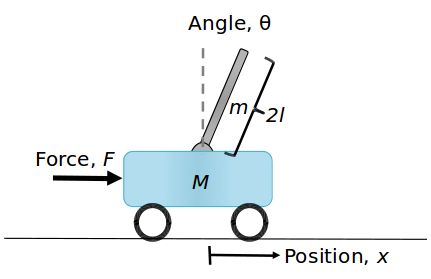
\includegraphics[width=5cm,keepaspectratio]{SystemDiagram.png}
 	\caption{System Diagram}
 	\label{fig:sys_diagram}
 \end{figure}
Using the above assumptions, we derived the non-linear equations of motion\footnote{The equations have no moment of inertia term because assumption (3) results in $J=\frac{1}{12}m(2l)^2$} using Newton's second law.  The description of the parameters and their values are given in Table \ref{table:paramvalues}.
\begin{equation}
\begin{aligned}
\frac{4}{3}l \ddot{\theta} &= g \sin \theta - \cos \theta \ddot{x} \\
(M+m)\ddot{x} &= F + ml \theta^2 \sin\theta -ml\ddot{\theta}\cos\theta
\end{aligned}
\label{eq:EOM_nonlinear}
\end{equation}
\begin{table}[h!]
 \centering
  \renewcommand{\arraystretch}{1.5}
 \begin{tabular}{ |c |c  |l |}
 \hline
 	 \textbf{Parameter} & \textbf{Value} & \textbf{Description}  \\ \hline
 	 M & 0.94 & Mass of the cart, kg \\ \hline
 	 m & 0.23 & Mass of the pole, kg \\ \hline
 	 l & 0.3302 & Distance along pole from pivot to center of mass, m \\ \hline
 	 g & 9.81 & Acceleration due to gravity, m/{sec\textsuperscript{2}} \\ \hline
 	 F & --- & Force applied to the cart, N \\ \hline
 	 x & --- & Cart position, m \\ \hline
 	 \.x & --- & Cart velocity, m/sec \\ \hline
 	 $\theta$ & --- & Angle of pole, rad \\ \hline
 	 $\dot\theta$ & --- & Angular velocity of pole, rad/sec \\ \hline
 \end{tabular}
 \caption{System Parameters (values from \cite{lab6})}
 \label{table:paramvalues}
 \end{table}
 \FloatBarrier
These can be rearranged into the nonlinear continuous-time first-order system of equations
\begin{equation}
\begin{aligned}
\matr{\dot{x}} &= \matr{f}(\matr{x},u),\quad  \matr{x} = \begin{bmatrix}
	x \\
	\dot{x} \\
	\theta \\
	\dot{\theta} \\
\end{bmatrix} \\
\matr{\dot{x}} &= \begin{bmatrix}
	\dot{x} \\
	\ddot{x} \\
	\dot{\theta} \\
	\ddot{\theta} \\
\end{bmatrix} = \begin{bmatrix}
\dot{x} \\
\frac{F+ml\dot{\theta}^2\sin\theta}{M+m} -\frac{ml\cos\theta}{m+M}\frac{mgl\sin\theta- \frac{ml}{M+m} F\cos\theta -\frac{m^2l^2}{m+M}\dot{\theta}^2\sin\theta\cos\theta}{\frac{4}{3}ml^2-\frac{m^2l^2}{M+m}\cos^2 \theta} \\[6pt]
\dot{\theta} \\
\frac{mgl\sin\theta - \frac{ml}{M+m} F\cos\theta -\frac{m^2l^2}{m+M}\dot{\theta}^2\sin\theta\cos\theta}{\frac{4}{3}ml^2-\frac{m^2l^2}{M+m}\cos^2 \theta }
\end{bmatrix}
\end{aligned}
\label{eq:nonlinear_ss_continuous}
\end{equation}
After rearranging into this form, the states of the system (the variables in vector $\matr{x}$) become evident. A description of each of the elements of the state vector is included in Table \ref{table:paramvalues}. No manipulation to the state equations is necessary since $\theta$, the critical output to be estimated, is already one of the states.\\

The original intention was to compare the performance of the estimators when using a single sensor to measure cart position (see Equation \ref{eq:singleoutput}) and two sensors for cart position and pole angular rate (see Equation \ref{eq:1output}). 
 \begin{align}
 y = \begin{bmatrix}
 1 & 0 & 0 & 0 \\
 \end{bmatrix} \begin{bmatrix}
 	x \\
 	\dot{x} \\
 	\theta \\
 	\dot{\theta} \\
 \end{bmatrix}
 \label{eq:singleoutput}
 \end{align}
 It was determined that cart position was the only state that could be measured by itself and result in a full-rank observability matrix, $\mathcal{O}$. However, significantly poor performance led to further analysis (See Appendix \ref{appendix:ctrb_obsv}) and it was determined that all subsequent estimators should be built using measurements from two states, one of which was the cart position. Pole angular rate was selected as the second measurement, resulting in the output equation:
\begin{align}
y = \begin{bmatrix}
1 & 0 & 0 & 0 \\
0 & 0 & 0 & 1
\end{bmatrix} \begin{bmatrix}
	x \\
	\dot{x} \\
	\theta \\
	\dot{\theta} \\
\end{bmatrix}
\label{eq:1output}
\end{align}

\subsection{Noise Characteristics}\label{ssecsensornoise}

A sensor was selected for each measured state, cart position and pole anglular velocity, while trying to balance accuracy and cost. For the cart position, the Garmin LIDAR-Lite v3 was selected for its accuracy of +/-2cm and retail cost of \$129.99\cite{lidarSensor}. The sensor noise was then approximated as Gaussian zero-mean with a standard deviation, $\sigma_{v_1}$, equal to the specificed accuracy. To measure the angular rate of the pole, an InvenSense ITG-3200 MEMS gyroscope was selected, and is available from SparkFun for \$24.99. The datasheet\cite{gyroSensor} specifies the RMS noise to be $0.38\frac{\circ{}}{sec}=0.0066\frac{rad}{sec}$, and RMS noise is equal to standard $\sigma_v$ deviation provided that the noise is zero-mean. These measurement noise parameters are summarized in Table \ref{table:sensorNoise}.

\begin{table}[h!]
 \centering
  \renewcommand{\arraystretch}{1.5}
 \begin{tabular}{ |c |c |}
 \hline
 	 \textbf{State} & \textbf{Measurement Noise Variance, }$\bm{\sigma_{v_i}^2}$  \\ \hline
 	 $x$ & 0.0004 \\ \hline
 	 $\dot{\theta}$ & 0.0000440 \\ \hline
 \end{tabular}
 \caption{System measurement noise characteristics.}
 \label{table:sensorNoise}
 \end{table}
If a real cart-pole system was built using the parameters in Table \ref{table:paramvalues}, one must simply look at the assumptions in Section \ref{section:systemDescription} to see that there are many potential sources of error. These sources of error could easily be justified as disturbances, otherwise known as process noise, which is a distribution of possible outcomes for the states of the system. Given that this project focuses entirely on simulation data, a method had to be developed for introducing process noise to the system. The method selected for this project was to inject process noise by assuming it came in through the system input. Therefore, an initial value of $\sigma_{w}^2=0.0004$ was selected (See Appendix \ref{appendix:processNoise} for details on how a value was quantified). \\
The process and measurement noise assumptions listed above can be summarized as
\begin{equation}
\begin{aligned}
\matr{w}_k &\sim \matr{N}\left(\begin{bmatrix}
0 \\
0 \\
0 \\
0
\end{bmatrix},\begin{bmatrix}
\sigma_w^2 & 0 & 0 & 0 \\
0 & \sigma_w^2 & 0 & 0 \\
0 & 0 & \sigma_w^2 & 0 \\
0 & 0 & 0 & \sigma_w^2
\end{bmatrix}\right) \\
\matr{v}_k &\sim \matr{N}\left(\begin{bmatrix}
0 \\
0
\end{bmatrix},\begin{bmatrix}
\sigma_{v_1}^2 & 0 \\
0 & \sigma_{v_2}^2 
\end{bmatrix}\right)
\end{aligned}
\end{equation}

\section{Estimators and Resulting Discretized State Space Models}
\subsection{Kalman Filter (KF)}
*Note best linear estimator
In order to implement a linear Kalman Filter, we will need to linearize these equations. Since the unstable portion of the system is directly related to the angle of the pole, it is our desire to keep the pole at the vertical position of 0$^\circ$. Therefore, this angle is the one about which we want to linearize; this is often called a "small angle approximation." This first-order truncation of the trigonometric Taylor series expansions results in the following substitutions to our nonlinear equations:
\begin{align*}
\sin \theta &\approx \theta \\
\cos \theta &\approx 1 \\
\dot{\theta}^2 &\approx 0
\end{align*}
Making these substitutions and rearranging the equations into matrix form results in the Linear State Space Model:
\begin{equation}
\begin{bmatrix}
	\dot{x} \\
	\ddot{x} \\
	\dot{\theta} \\
	\ddot{\theta} \\
\end{bmatrix} = \begin{bmatrix}
0 & 1 & 0 & 0 \\
0 & 0 & -\frac{-m^2l^2g}{\gamma} & 0 \\
0 & 0 & 0 & 1\\
0 & 0 & \frac{(M+m)mgl}{\gamma} & 0
\end{bmatrix} \begin{bmatrix}
	x \\
	\dot{x} \\
	\theta \\
	\dot{\theta} \\
\end{bmatrix}  + \begin{bmatrix}
0 \\
\frac{J+ml^2}{\gamma} \\
0 \\
-\frac{ml}{\gamma}
\end{bmatrix} F
\label{eq:ss_continuous}
\end{equation}
where, 
\begin{align*}
\gamma &= J(M+m)+mMl^2 \\
J &= \frac{1}{3}ml^2
\end{align*}
This equation, when placed alongside the output equation (Equation \ref{eq:1output}), is a representation of the familiar linear state-space form
\begin{equation*}
\begin{aligned}
\matr{\dot{x}} &= \matr{A}\matr{x} + \matr{B}u \\
\matr{y} &= \matr{C}\matr{x}
\end{aligned}
\end{equation*}

After substituting the parameter values and discretizing the model\footnote{The Matlab function expm() was used to convert \textbf{A\textsubscript{c}} to \textbf{A} using the appropriate equation and \textbf{B\textsubscript{c}} to \textbf{B}. The MATLAB function c2d() was also used to confirm our results.}, 
the resulting Discretized Linear State Space Model is:

\begin{equation}
\begin{bmatrix}
x_{k+1} \\
\dot{x}_{k+1} \\
\theta_{k+1} \\
\dot{\theta}_{k+1}
\end{bmatrix}
=
\begin{bmatrix}
1 & 0.02 & -3.39e-4 & -2.26e-6\\
0 & 1 & -3.39e-2 & -3.39e-4\\
0 & 0 & 1.0052 & 2.0035e-2\\
0 & 0 & 0.52308 & 1.0052\\
\end{bmatrix}
\begin{bmatrix}
x_{k} \\
\dot{x}_{k} \\
\theta_{k} \\
\dot{\theta}_{k}
\end{bmatrix}
+
\begin{bmatrix}
1.7097e-4\\
1.7099e-2\\
-4.5581e4\\
-4.562e-2\\
\end{bmatrix}
F
\label{eq:linear_discrete}
\end{equation}
\subsubsection{Stability Analysis}
The intuition that the system is unstable can be verified by checking the stability criterion
\begin{equation}
|\vec{\lambda}(\matr{A})| < \vec{1}
\end{equation}
which says that all of the eigenvalues of the system must be less than 1 for the system to be stable. The discrete-time linear system eigenvalues are found using the MATLAB command eig(A) to be
\begin{equation}
\vec{\lambda} = \begin{bmatrix}
    1.0000 \\
    1.0000 \\
    1.1076 \\
    0.9029
\end{bmatrix}
\end{equation}
which does not meet the stibility criterion, confirming intuition.  The system is controllable and observable (See Appendix \ref{appendix:ctrb_obsv} for details), and because the system is observable it is also detectable.  The system only needs to be detectable for the KF.

\subsection{Extended Kalman Filter (EKF)}
The Extended Kalman Filter (EKF) differs from the KF by utilizing the nonlinear discrete time state equations in place of the linear equations. This is accomplished by inserting the \textit{a posteriori} estimates of the states from the previous time step into the discrete nonlinear equations to get the \textit{a priori} estimates of the states at the current time step. This necessitates that the the nonlinear discrete time equations be computed. This is accomplished using the first-order Euler approximations of the continuous time equations (Equation \ref{eq:nonlinear_ss_continuous}):
\begin{equation}
\begin{aligned}
\matr{x}_{k+1} &= \matr{f}_k (\matr{x}_k,u_k) \\
\begin{bmatrix}
x_{k+1} \\[8pt]
\dot{x}_{k+1} \\[8pt]
\theta_{k+1} \\[8pt]
\dot{\theta}_{k+1}
\end{bmatrix} &= \begin{bmatrix}
x_k + \dot{x}_k \Delta t \\
\dot{x}_k + \biggr(\frac{F+ml\dot{\theta}_k^2\sin\theta_k}{M+m} -\frac{ml\cos\theta_k}{m+M}\frac{mgl\sin\theta_k- \frac{ml}{M+m} F\cos\theta_k -\frac{m^2l^2}{m+M}\dot{\theta}_k^2\sin\theta_k\cos\theta_k}{\frac{4}{3}ml^2-\frac{m^2l^2}{M+m}\cos^2 \theta_k}\biggr) \Delta t  \\
\theta_k + \dot{\theta}_k \Delta t \\
\dot{\theta}_k + \biggr(\frac{mgl\sin\theta_k - \frac{ml}{M+m} F\cos\theta_k -\frac{m^2l^2}{m+M}\dot{\theta}_k^2\sin\theta_k\cos\theta_k}{\frac{4}{3}ml^2-\frac{m^2l^2}{M+m}\cos^2 \theta_k}\biggr) \Delta t
\end{bmatrix}
\end{aligned}
\label{eq:nonlinear_discrete}
\end{equation}
Next, the Jacobian of Equation \ref{eq:nonlinear_discrete} will be evaluated at each time step:
\begin{align}
\begin{aligned}
\matr{A'}_{k-1} &= \matr{J}\bigr|_{\hat{\matr{x}}_{k-1|k-1}} \\
&= \begin{bmatrix}
1 & \Delta t & 0 & 0 \\[8pt]
0 & 1 & \frac{\partial \dot{x}_{k+1}}{\partial \theta_k}\Big|_{\hat{\matr{x}}_{k-1|k-1}}\Delta t & \frac{\partial \dot{x}_{k+1}}{\partial \dot{\theta}_k}\Big|_{\hat{\matr{x}}_{k-1|k-1}}\Delta t \\[8pt]
0 & 0 & 1 & \Delta t \\[8pt]
0 & 0 & \frac{\partial \dot{\theta}_{k+1}}{\partial \theta_k}\Big|_{\hat{\matr{x}}_{k-1|k-1}}\Delta t & 1+\frac{\partial \dot{\theta}_{k+1}}{\partial \dot{\theta}_k}\Big|_{\hat{\matr{x}}_{k-1|k-1}}\Delta t
\end{bmatrix}
\end{aligned}
\label{eq:jacobian_EKF}
\end{align}
where,
\begin{align*}
\frac{\partial \dot{\theta}_{k+1}}{\partial \theta_k}\Big|_{\hat{\matr{x}}_{k-1|k-1}} &= \
\frac{(mgl\cos\theta + \frac{ml}{M+m}u_k\sin\theta_k - \frac{m^2l^2}{M+m}\dot{\theta}_k^2(\cos^2\theta_k-\sin^2\theta_k))den - num(2\frac{m^2l^2}{M+m}\cos\theta_k\sin\theta_k)}{den^2} \\
\frac{\partial \dot{\theta}_{k+1}}{\partial \dot{\theta}_k}\Big|_{\hat{\matr{x}}_{k-1|k-1}} &=\
-\frac{\frac{2m^2l^2}{M+m}\dot{\theta}_k\sin\theta_k\cos\theta_k}{den} \\
\frac{\partial \dot{x}_{k+1}}{\partial \theta_k}\Big|_{\hat{\matr{x}}_{k-1|k-1}} &=\
-\frac{ml}{M+m}(-\sin\theta_k \frac{num}{den} + \cos\theta_k\frac{\partial \dot{\theta}_{k+1}}{\partial \theta_k}\Big|_{\hat{\matr{x}}_{k-1|k-1}}) + \frac{ml}{M+m}\dot{\theta}_k\sin\theta_k \\
\frac{\partial \dot{\theta}_{k+1}}{\partial \dot{\theta}_k}\Big|_{\hat{\matr{x}}_{k-1|k-1}} &=\
-\frac{ml}{M+m}\cos\theta_k\frac{\partial \dot{\theta}_{k+1}}{\partial \dot{\theta}_k}\Big|_{\hat{\matr{x}}_{k-1|k-1}} + \frac{2ml}{M+m}\dot{\theta}_k\sin\theta_k \\
num &= mgl\sin\theta_k - \frac{ml}{M+m} F\cos\theta_k -\frac{m^2l^2}{M+m}\dot{\theta}_k^2\sin\theta_k\cos\theta_k \\
den &= \frac{4}{3}ml^2-\frac{m^2l^2}{M+m}\cos^2 \theta_k
\end{align*}
and all references to state variables from time step $k$ are inserted from the $k-1$ previous time step estimate.
Using Equation \ref{eq:jacobian_EKF}, the \textit{a priori} covariance update, $\matr{P}_{k|k-1}$, is computed as
\begin{equation}
\matr{P}_{k|k-1} = \matr{A}'_{k-1} \matr{P}_{k-1|k-1} {\matr{A}'}_{k-1}^T + \matr{Q}
\end{equation}
The rest of the algorithm follows the same process as the linear Kalman Filter.\footnote{Although it is not true in general that the EKF measurement update follows the same process as KF, the absence of nonlinearities in the system output equation, along with unity coefficients (no scaling) on the process and measurement noise, results in the EKF \textit{a posteriori} estimate following exactly the KF \textit{a posteriori} algorithm.}
\subsection{Unscented Kalman Filter (UKF)}
When the nonlinearity of a dynamic model is severe, the state estimations propagated through linearized model will not be accurate. Though EKF incorporates a nonlinear model in model prediction, it still uses a local linearized dynamic model ${\matr{A}'}$ to estimate the variance matrix $\matr{P}_{k|k}$ at each time step. However, the Unscented Kalman Filter (UKF) has been shown to have better accuracy of the mean and the variance of state estimation compared to the EKF, especially in severely nonlinear dynamic models. In the UKF, the mean and the variance are estimated based on a sampling method. The implementation of the UKF for this project was based on a paper by Moireau and Chapelle \cite{moireau2011reduced}. In model prediction, 2n sample points were selected ($\sigma$ points) based on the current knowledge of the state estimation $\matr{\hat{X}_{k-1|k-1}}$ and $\matr{\hat{P}_{k-1|k-1}}$. The 2n sampling points are shown in Equations \ref{eq:UKF1} and \ref{eq:UKF2}.
\begin{equation}
	\hat{\matr{X}}^{(i)}_{k-1|k-1}+(\sqrt{n\matr{P}_{k-1|k-1}}),\  i=1,2,...n
\label{eq:UKF1}
\end{equation}
\begin{equation}
 \hat{\matr{X}}^{(i)}_{k-1|k-1}-(\sqrt{n\matr{P}_{k-1|k-1}}),\  i=1,2,...n
\label{eq:UKF2}
\end{equation}
The nonlinear discrete model from Equation \ref{eq:nonlinear_discrete} is used to propagate each $\sigma$ points to get the state estimations $\hat{X}_{k|k-1}$. Then the mean and the variance of propagated sample points are calculated to obtain $\hat{\matr{X}}_{k|k-1}$ and $\hat{\matr{P}}_{k|k-1}$ using Equations \ref{eq:UKF3} and \ref{eq:UKF4}.
\begin{equation}
 \hat{\matr{X}}_{k|k-1}=\frac{1}{2n}\sum_{i}^{2n}\hat{\matr{X}^{(i)}_{k|k-1}}
\label{eq:UKF3}
\end{equation}
\begin{equation}
\hat{\matr{P}}_{k|k-1}=\frac{1}{2n}\sum_{i}^{2n}(\hat{\matr{X}^{(i)}_{k|k-1}}-\hat{\matr{X}_{k|k-1}})(\hat{\matr{X}^{(i)}_{k|k-1}}-\hat{\matr{X}_{k|k-1}})^T + \matr{Q}_{k-1}
\label{eq:UKF4}
\end{equation}
Notice that the estimation of process noise is still added at each step of model prediction. Therefore the variance will not converge for open loop estimation. The measurement update follows steps similar to the unscented transformation in model prediction, but uses the measurement function $h_k(x)$ to propagate 2n $\sigma$ points to obtain 2n estimated measurement points using the output state space function. Then the mean, variance $\matr{P}_y+\matr{R}_k$ and covariance $\matr{P}_{xy}$ of transformed $\sigma$ points are calculated.  The posterior state estimation can then be obtained from Equations \ref{eq:UKF5} and \ref{eq:UKF6}.
\begin{equation}
	\hat{\matr{X}}_{k|k} = 	\hat{\matr{X}}_{k|k-1} + \matr{P}_{xy} \matr{P}^{-1}_{y}(\matr{y_k}-\hat{\matr{y}}_{k|k-1})
\label{eq:UKF5}
\end{equation}
\begin{equation}
	\matr{P}_{k|k}=	\matr{P}_{k|k-1} - \matr{P}_{xy}\matr{P}^{-1}_{y}\matr{P}_{xy}^T
\label{eq:UKF6}
\end{equation}
\section{Methodology and Test Cases} 
The general system architecture of an inverted pendulum is shown as a block diagram in Figure \ref{fig:block_diagram}. Given the initial state $X_0$, the LQR (Linear Quadratic Regulator) controller  calculates the optimal input force, $F_1$, to inverted pendulum system for the current time step. The system responds to the input and output actual state $\matr{X}_1$ at next time step. The sensor measurement will output state measurements, $\matr{y}_1$, that include noise. The input, $F_1$, and measurements, $\matr{y}_1$, are used as inputs to estimator and then the output estimated states, $\matr{\hat{X}}_2$, are given to controller to calculate optimal input, $F_2$, in time step $t_2$.  The controller will calculate the optimal force only based on estimated states. The controller parameters are not tuned for different estimators in order to show the performance of different estimators in the real time system. 
\begin{figure}[h!]
	\centering
	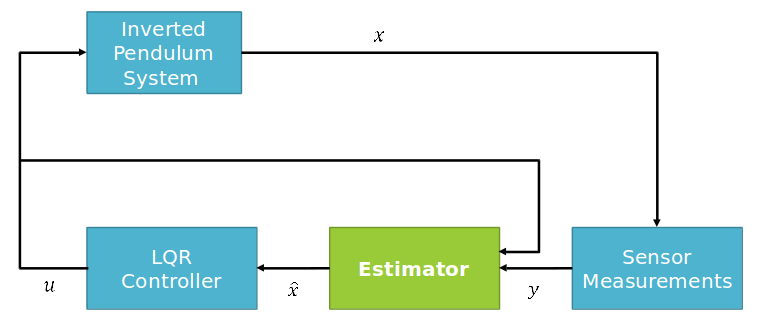
\includegraphics[width=10cm,keepaspectratio]{SystemArchitecture.png}
	\caption{Block diagram of our system}
	\label{fig:block_diagram}
\end{figure}

\subsection{Simulation description}
The purpose of the simulator is to generate ground truth (i.e. actual states), input, and measurement data for use in offline test cases, as well as for online comparison of estimators.  For the offline test cases, all the estimators recieve the same input and allows a more direct comparison. The simulator used in this project is based on the general system architecture (See Figure \ref{fig:block_diagram}) and contains modifications (See Appendix xx).  The simulation is modeled from a simulator in OpenAI Gym \cite{OpenAI}. The parameters of the system and input constraints were modified to reflect an actual inverted pendulum system \cite{lab6}. Process noise and measurement noise are also included based on the analysis discussed in Section \ref{ssecsensornoise}.  The animation produced by the simulator is shown in Figure \ref{fig:simulator}.
\begin{figure}
	\centering
	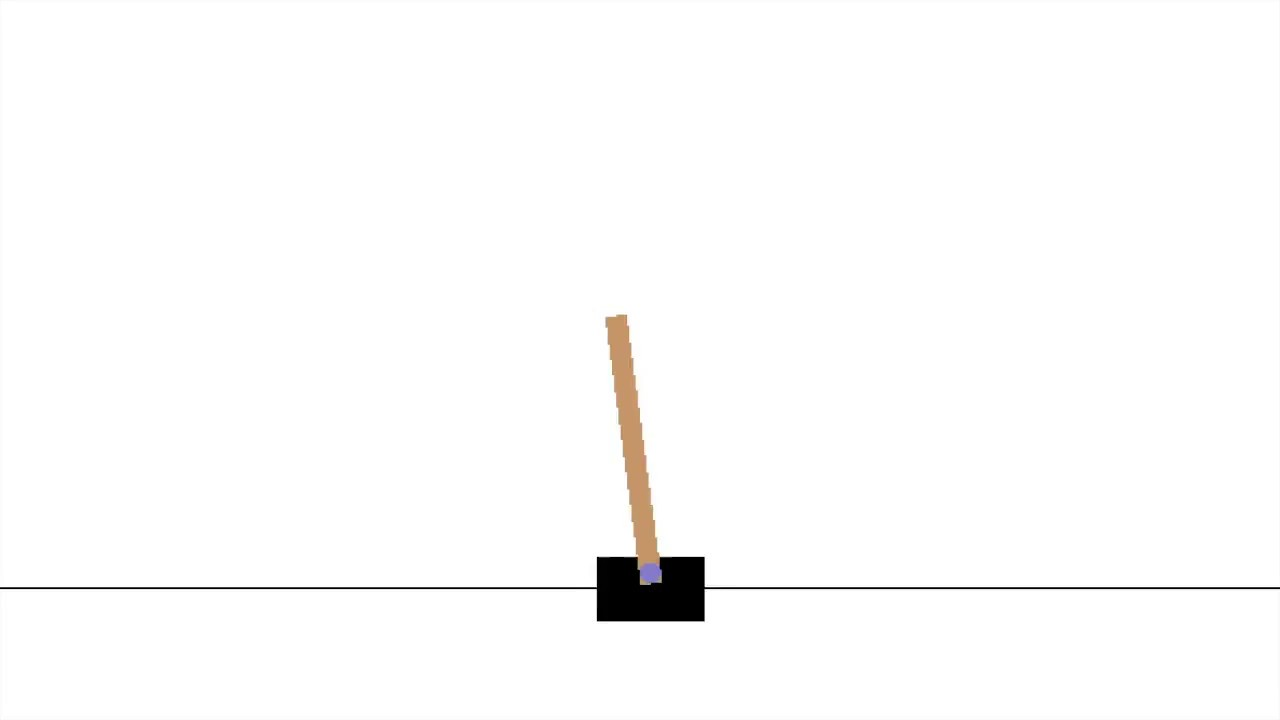
\includegraphics[width=10cm,keepaspectratio]{Simulator.jpg}
	\caption{Example of Animation Frame Produced by Simulator}
	\label{fig:simulator}
\end{figure}
\subsection{Expected results}
The whole simulation running based on discretized nonlinear system following Equations \ref{eq:nonlinear_discrete}. In small starting angles ($\theta<10^o$), the nonlinearity of system is not very severe, so the performance of KF should work fine. The estimated error of three estimators can be comparable. However, when the starting angle is increased, the linearity error of linearized system around equilibrium position will rise. As a result, KF will not perform well, while EKF and UKF will work much better in nonlinear case. For online testing, estimating states of KF in large starting angle condition will fail the controller, while EKF and UKF still get controller to work fine. Likewise, in offline testing, the estimated error of KF will be larger than UKF and EKF in large starting angle of our system.
\section{Results}
\subsection{Offline Results}

The offline test cases were constructed to evaluate linear and nonlinear estimator performance for various conditions regarding the number of sensor measurements, starting pole angle and tuning.
\begin{table}[h!]
 \centering
 \renewcommand{\arraystretch}{1.5}
 \begin{tabular}{ |l |c  |c |c |}
 \hline
 	 \textbf{Estimator} & \textbf{KF} & \textbf{EKF} & \textbf{UKF} \\ \hline
 	 \textbf{Pole Starting Angles}  & \multicolumn{3}{|c|}{5$^{\circ}$, 15$^{\circ}$, 60$^{\circ}$} \\ \hline
 	 \textbf{Sensors} & x; x and $\dot\theta$ & \multicolumn{2}{|c|}{x and $\dot\theta$} \\ \hline
 	 \textbf{Q Scaling}  & \multicolumn{3}{|c|}{Q, 0.001Q, 0.1Q, 10Q} \\ \hline
 \end{tabular}
 \caption{Offline Test Cases}
 \label{table:offlinecases}
 \end{table}
The comparison varying the number of sensors was restricted to the KF because the results made it clear that a single sensor had poor performance, as seen in Figure \ref{fig:sensorsKF}.  The results did demonstrate that additional sensors will improve results, even if a sensor is noisy.  In this case, the addition of a second sensor improves the pole angle estimation and it follows the ground truth well.  All of the following test cases used two sensors.
\begin{figure}[h!]
 	\centering
 	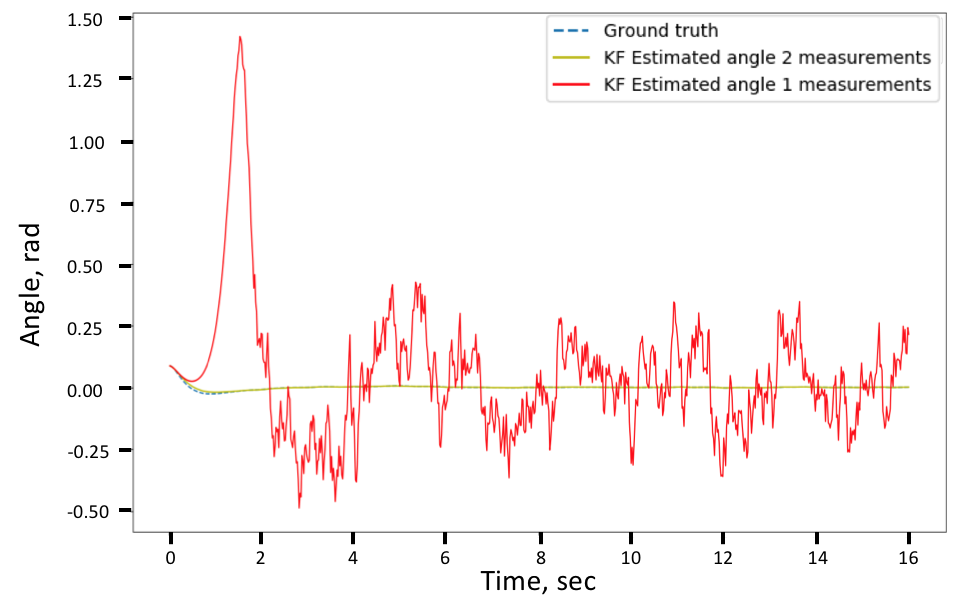
\includegraphics[width=10cm,keepaspectratio]{SensorsKF.png}
 	\caption{Comparison of KF Results for a Single Sensor and Two Sensors (Pole starting angle = 5$^{\circ}$, Scaling = Q)}
 	\label{fig:sensorsKF}
 \end{figure}
 
 The next test case compared the use of linear (KF) and nonlinear estimators (EKF) for a small starting pole angle ($\theta$ = 5$^{\circ}$).  As seen in Figure \ref{fig:5degKFvEKF}, the EKF follows the ground truth closer than the KF and the difference is likely due to the linearization errors in the KF.  The performance of the KF is relatively close to the EKF, as their RMSE is the same order of magnitude, 9.86 x 10$^{-4}$ rad and 3.10 x 10$^{-4}$ rad, respectively.
 \begin{figure}[h!]
 	\centering
 	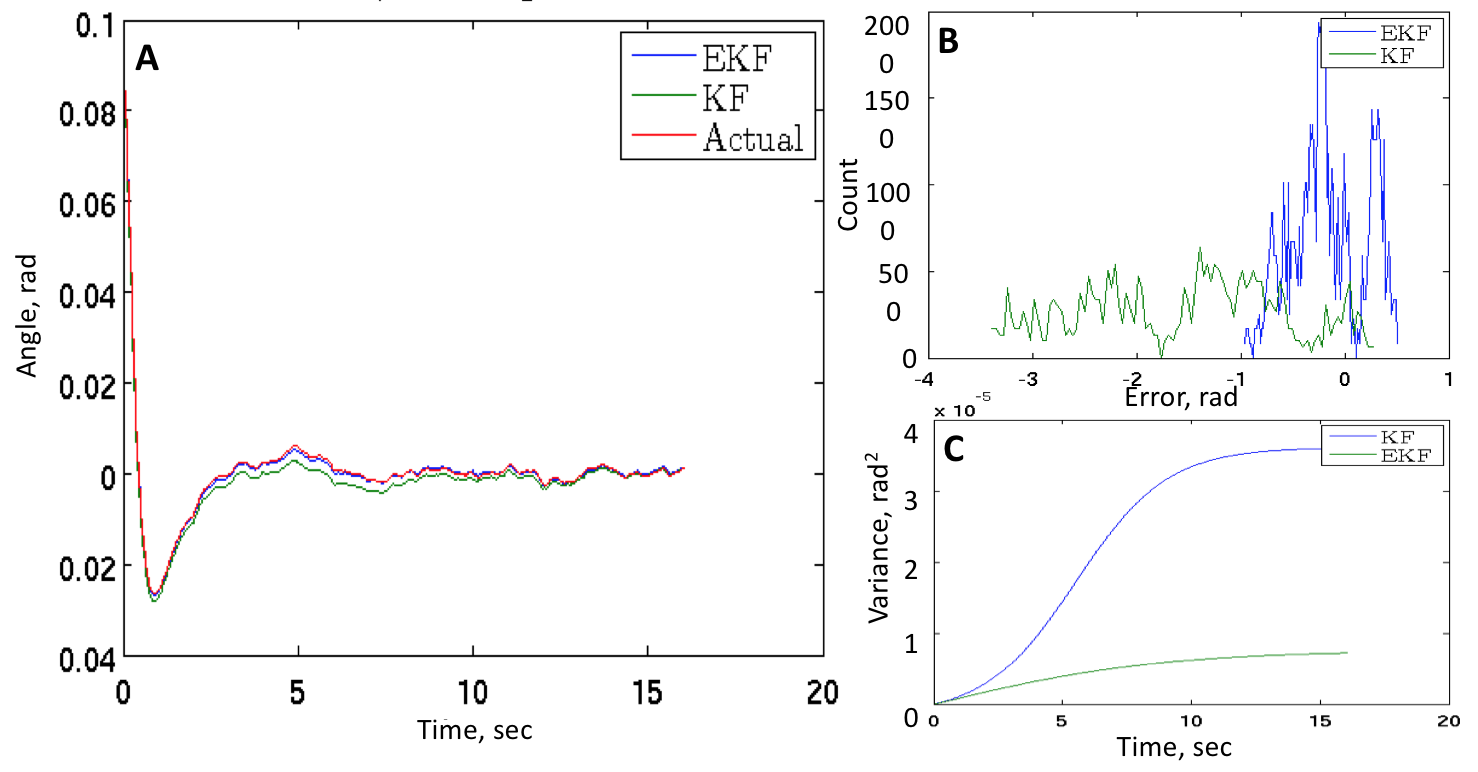
\includegraphics[width=15cm,keepaspectratio]{5degKFvEKF.png}
 	\caption{Comparison of KF and EKF (Pole starting angle = 5$^{\circ}$, Scaling = Q). \textbf{A} Estimation of pole angle \textbf{B} Error distribution \textbf{C} Estimated variance of the estimation}
 	\label{fig:5degKFvEKF}
 \end{figure}

 The subsequent test case introduced an additional nonlinear estimator, UKF, and increased the staring pole angle ($\theta$ = 15$^{\circ}$).  In Table \ref{table:rmse}, the estimator performance is assessed by RMSE and the test case run time (i.e. the total time to go through the one test case), where smaller RMSE and run times are better.  The KF RMSE is an order of magnitude larger for all tuning conditions compared to the nonlinear estimators.  As opposed to the test case where the pole starting angle was 5$^{\circ}$, the linearization errors in the KF are affecting its performance enough that it significantly deviates from the nonlinear estimators.  However, the test case run time is an order of magnitude smaller.  The EKF and UKF score similarly for RMSE, but the UKF test case run time is doubled.  This result is expected due to the computational cost of running the UKF.
 \begin{table}[h!]
 \centering
 \renewcommand{\arraystretch}{1.5}
\begin{tabular}{|c|c|c|c|c|}
	\hline
	\multirow{2}{*}{\textbf{Estimator}} & \multicolumn{3}{c|}{\textbf{RMSE, rad}} & \textbf{Test Case Run Time, sec} \\ \cline{2-5}
	& Q & 0.1Q & 10Q & Q \\ \hline
	\textbf{KF} & 0.00148 & 0.0072 & 0.00883 & 0.063 \\ \hline
	\textbf{EKF} & 0.00030 & 0.000402 & 0.000412 & 0.230 \\ \hline
	\textbf{UKF} & 0.00029 & 0.000303 & 0.000304 & 0.426 \\ \hline
\end{tabular}
 \caption{Performance Comparison Across Estimators for a Pole Starting Angle $\theta$ = 15$^{\circ}$}
 \label{table:rmse}
 \end{table}
 
 The final offline test case used a large pole starting angle ($\theta$ = 60$^{\circ}$), which was well beyond the expected limits of the KF.  As shown in Figure \ref{fig:offline60deg} the nonlinear estimators track the ground truth well, whereas the KF has relatively large deviations, particularly as the pole changes direction.  The distribution of errors for the nonlinear estimators appear normally distributed.  The KF error distribution has a slight tail, but appeared relatively normally distributed.  The KF was able to bring the pole to an equilibrium above the pivot point during an offline case.  However, that was not the result during online testing and is discussed in Section \ref{ssec:LargeAngleOnline}.
  \begin{figure}[h!]
 	\centering
 	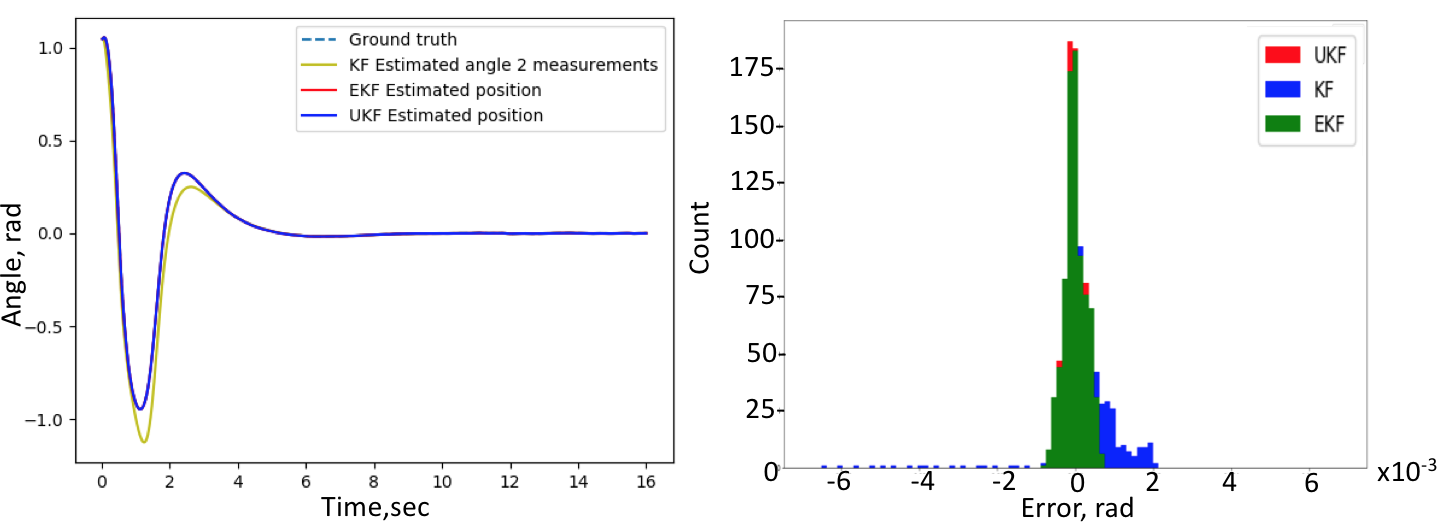
\includegraphics[width=15cm,keepaspectratio]{offline60deg.png}
 	\caption{Comparison of KF, EKF and UKF (Pole starting angle = 60$^{\circ}$, Scaling = 0.001Q). \textbf{A} Estimation of pole angle \textbf{B} Error distribution}
 	\label{fig:offline60deg}
 \end{figure}

\subsection{Online Results}
\subsubsection{KF, EKF for large angles} \label{ssec:LargeAngleOnline}
With two sensor measurements, both KF and EKF work fine to stabilize the system around equilibrium position. However, if we decrease estimation of process noise estimation Q, which means to trust dynamic model more in estimation, we found that KF will not generate desired estimates to make the controller come to stable position. The online running result for KF and EKF is shown in Figure \ref{fig:onlineKFvsEKF}. 
\begin{figure}[h!]
	\centering
	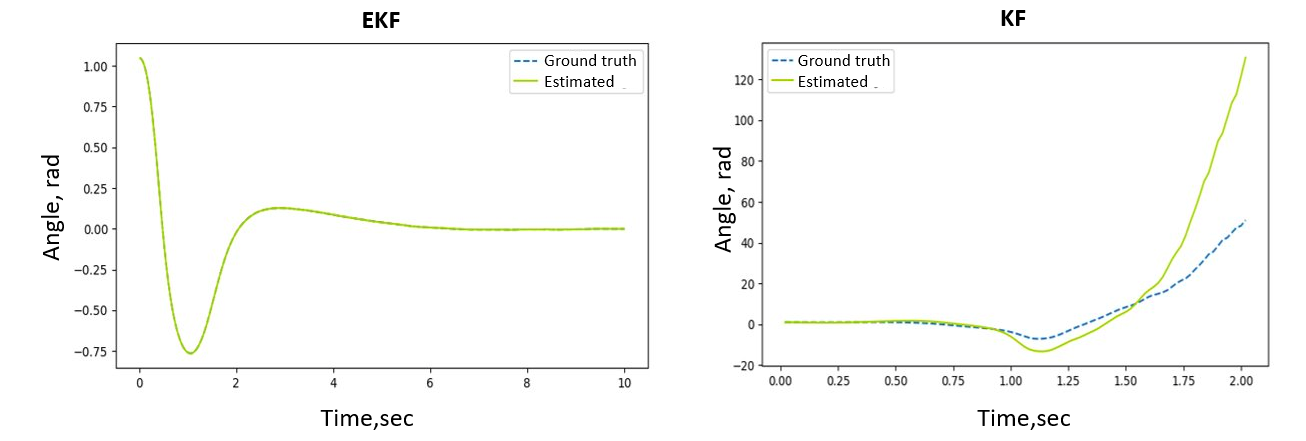
\includegraphics[width=15cm,keepaspectratio]{EKFvsKF_online.png}
	\caption{Online result of EKF and KF}
	\label{fig:onlineKFvsEKF}
\end{figure}

From figure, we can find that EKF still works pretty good when we set smaller Q, however, the KF works poorly and it proves that high linearity error for KF estimator.
\subsubsection{Successful cases working online}
In simulation, with different estimators, starting angles and sensors, multiple experiments are running to show the online performances of estimator. In the table \ref{table:offlinecases}, the largest starting angles are searched for online experiments. We can find that two measurements can greatly improve the estimation accuracy. However, when sensor measurements are not reliable, accurate model are needed to improve the estimation accuracy.
\begin{table}[h!]
	\centering
	\renewcommand{\arraystretch}{1.5}
	\begin{tabular}{ |l |c  |c |c | c|}
		\hline
		\multirow{2}{*}{\textbf{Estimators}} & \multicolumn{2}{|c|}{\textbf{One Measurement}} & \multicolumn{2}{|c|}{\textbf{Two Measurements}} \\ \cline{2-5}
		& $\sigma = 0.02$ & $\sigma=0.004$(self tuning) & $\hat{Q} = Q$ & $\hat{Q} = 0.001Q$ \\ \hline
		\textbf{KF} & None & $10^\circ{}$ & $60^\circ{}$ & $45^\circ{}$ \\ \hline
		\textbf{EKF} & None & $30^\circ{}$ & $63^\circ{}$ & $63^\circ{}$ \\ \hline
		\textbf{UKF} & None & $30^\circ{}$ & $63^\circ{}$ & $63^\circ{}$ \\ \hline
	\end{tabular}
	\caption{Largest starting angle for various Online Test Cases and estimators}
	\label{table:offlinecases}
\end{table}


\section{Conclusions}

This project sought to investigate the performance of three estimators--the linear Kalman Filter (KF), the nonlinear Extended Kalman Filter (EKF), and the nonlinear Unscented Kalman Filter (UKF)--under varying conditions for an unstable, nonlinear system.  The conditions included the number of sensors, the pole starting angle, and the tuning of estimated noise variance.  Measures used were RMSE, test case run time, and the ability of the estimator to stablize the system online.  The conclusions from this project are as follows:

\textbf{Offline Results:}
\begin{enumerate}
\item The single sensor selected was not sufficient to accurately estimate the pole angle, but the results did illustrate the the addition of sensors improves state estimation.  All subsequent test cases used two sensors.
\item The KF performed comparably to a nonlinear estimator, the EKF, for the small starting pole angle ($\theta$ = 5$^{\circ}$).
\item The KF performance deviated from the nonlinear estimators, the EKF and the UKF, for a starting pole angle of 15$^{\circ}$, as measured as RMSE.  The KF could not be tuned to outperform the nonlinear estimators.  The results from tuning verified that a perfect estimate of the noise variance will yield the best estimation results, and over- or underestimation will result in larger errors.  The test case run time was the shortest for KF and longest for UKF.
\item While the KF could track the ground truth and bring the system to an equilbruim for a large starting pole angle ($\theta$ = 60$^{\circ}$), the result was only applicable offline.  The nonlinear estimators need to be used for large starting pole angles.
\end{enumerate}

\textbf{Online Results:}
\begin{enumerate}
\item It was possible for a single sensor to work during online applications, if the sensor measurement accuracy was an order of magnitude better.  Using a more accurate sensor, the KF can perform online for starting pole angles up to 10$^{\circ}$ and 30$^{\circ}$ for the nonlinear estimators.
\item When the model noise statistics are perfectly guessed, the KF can perform online for starting pole angles up to 60$^{\circ}$ and 63$^{\circ}$ for the nonlinear estimators.
\item When the model is trusted more, the KF can perform online for starting pole angles up to 45$^{\circ}$ and 63$^{\circ}$ for the nonlinear estimators.
\item In all cases, the nonlinear estimators can accomodate larger starting pole angles than the KF.
\end{enumerate}

Overall, the project results supported the initial hypotheses and the estimators generally behaved as expected.  One surprising result was the inability of the selected single sensor to work, but further investigation yielded a reasonable explanation.  It was also unexpected that the KF could run online with a starting pole angle of up to 45$^{\circ}$, which is beyond the small angle approximation limits, but demonstrates that the KF is the best linear estimator.  The implementation of process noise was a considerable challenge that resulted in a deeper understanding of the system.  It also highlighted the difficulties in estimating process noise a priori and the purpose of tuning.  This project demonstrated several concepts from the course and was a valuable learning experience.

\section{References}

%\cite{*}
\bibliography{references}{}
\bibliographystyle{ieeetr}

\pagebreak
\section{Appendices}
\subsection{Controllability and Observability}\label{appendix:ctrb_obsv}
\label%latex
To check observability $\mathcal{O}$ and controllability $\mathcal{C}$, we constructed their respective matrices from the linear discrete time state space model using
\begin{equation}
\mathcal{C} = \begin{bmatrix}
B & AB & A^2B & A^3B
\end{bmatrix} = \begin{bmatrix}
    0.0003 &   0.0009  &  0.0015   & 0.0021 \\
    0.0300  &  0.0300  &  0.0300   & 0.0301 \\
   -0.0005   &-0.0014  & -0.0023   &-0.0033 \\
   -0.0456  & -0.0461  & -0.0471   &-0.0485
\end{bmatrix}
\end{equation}
A quick check with MATLAB using the command rank($\mathcal{C}$) tells us $\mathcal{C}$ is rank(4), which by the textbook definition makes this system controllable. \\

Our initial attempt at using a Kalman filter with just one measurement (cart position) was not working very well. We then determined to check the observability matrix $\mathcal{O}$, defined as
\begin{equation}
\mathcal{O} = \begin{bmatrix}
C \\
CA \\
CA^2 \\
CA^3
\end{bmatrix}
\end{equation}

This matrix was also full rank, which was perplexing. Professor Lin then suggested that we check the condition number of the observability matrix. Using the MATLAB command cond(), we evaluated cond($\mathcal{O}$) = $6.67e+5$, which suggests that the observability matrix is almost singular. I think you and Sarah need to collaborate for the This was the source of some of our problems in implementing our state estimators. Based on this information, we attempted to add another sensor at the pole angular rate. After doing this, the condition number of the observability matrix was $60.437$, a much more reasonable number.
\subsection{Details of Process Noise}\label{appendix:processNoise}
Process noise was injected to the system through the input force. A motor model was constructed and with constant, linear coefficients of system variables. From this model,the input force was assumed to follow a linear relation with controlling voltage of motor circuit shown as Figure \ref{fig:circuit}.
\begin{figure}[h!]
	\centering
	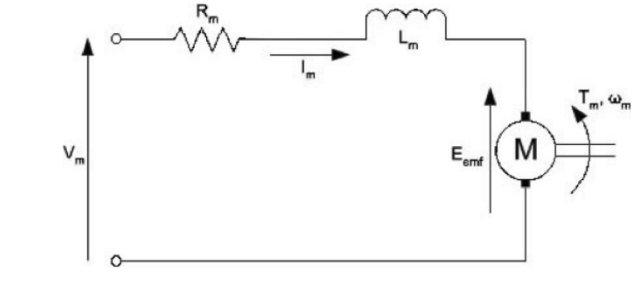
\includegraphics[width=10cm,keepaspectratio]{circuit.png}
	\caption{controlling circuit of motors}
	\label{fig:circuit}
\end{figure}
The linear relationship between force noise and motor voltage input noise\footnote{A value for $\alpha$ was selected based on small motors comparable to what would be required for a small cart-pole robot. \cite{lab3} acted as a guide and assisted with construction of a motor model.} is expressed as Equation \ref{FvsV}, $\alpha \approx 1.72$. It was assumed that the motor driver operates and 12 Volts and with a 10 bit DAC accuracy. By this analysis, the standard deviation $\sigma$ of the input noise can be approximated as $\alpha\frac{12}{2^{10}}$ = 0.02.
\begin{equation}
F = \alpha V + B
\label{FvsV}
\end{equation}
\subsection{Details of Controller}
In simulator, we use a discretized Linear Quadratic Regulator to output desired force at each time step. The idea is to use dynamic programming methodology to do backward recursion calculation starting from final position we want to get. At each step, with linear constraint and quadratic objective function, the desired force can be calculated by gradient method. Then the controller will choose first step of calculated force as input of system at current time step. The calculation for loop is shown in Figure \ref{fig:iLQR} \cite{puterman2014markov}.
\begin{figure}[h!]
	\centering
	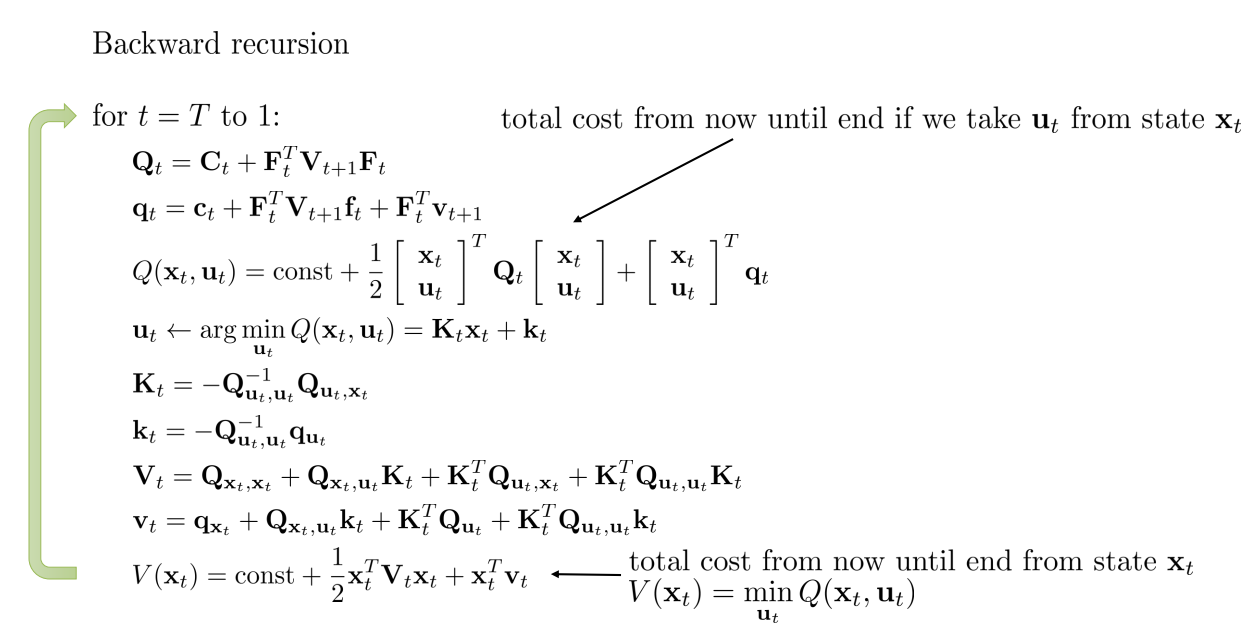
\includegraphics[width=15cm,keepaspectratio]{LQR.png}
	\caption{iterative Linear Quadratic Regulator (iLQR)}
	\label{fig:iLQR}
\end{figure}
\subsection{Discussion of Simulation Environment, Online versus Offline}
\begin{figure}[h!]
	\centering
	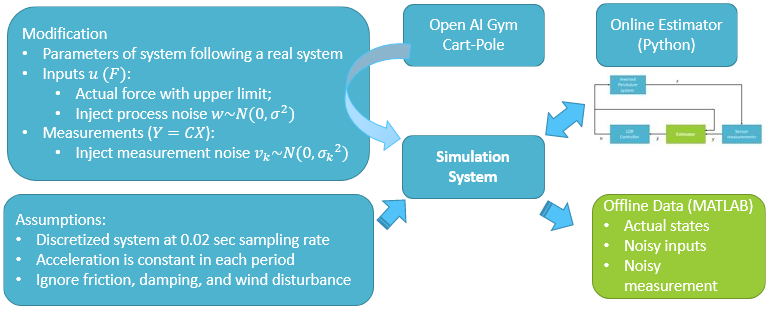
\includegraphics[width=10cm,keepaspectratio]{Simulation.png}
	\caption{High-level overview of simulation environment}
	\label{fig:simulation}
\end{figure}
The method of simulation can be ascertained by a study of Figure \ref{fig:simulation}. The offline ground truth data was generated by inserting parameters and initial conditions to the Python OpenAI Gym package. Then, this data was loaded into MATLAB for offline estimator performance comparison. \\

It was important to perform both offline and online estimation for several reasons. First, solely performing online estimation does not provide the designer with sufficient details regarding how and when state estimation errors become significant. Also, solely performing offline estimatoin doesn't paint a complete picture. Online performance of the linear KF was better than predictions based on offline estimators. \\
\begin{figure}[h!]
	\centering
	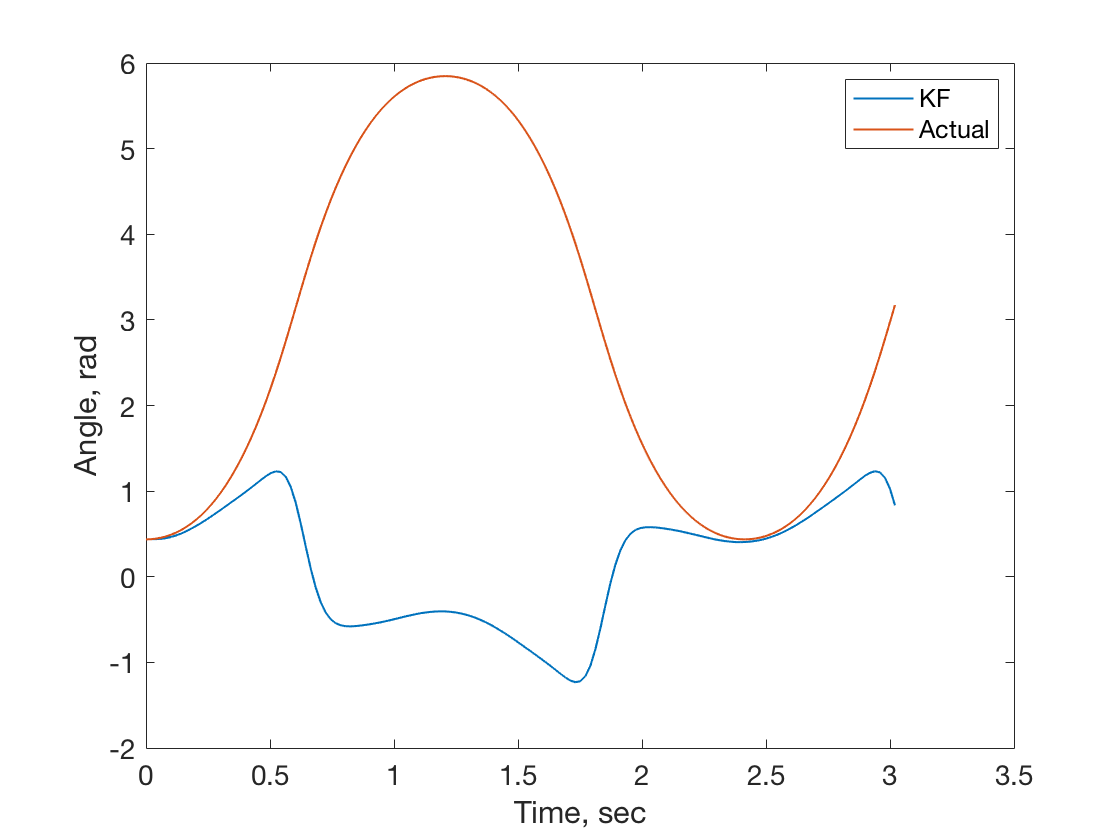
\includegraphics[width=10cm,keepaspectratio]{NoForcingOpen.png}
	\caption{Kalman Filter estimation of pole angle for a small initial angle and no input force}
	\label{fig:NoForcing}
\end{figure}

As an example, Figure \ref{fig:NoForcing} shows a short duration offline simulation of actual pole angle compared with its state estimation. From this image, it is shown that the nonlinearities of the cart-pole system become signifcant at relatively small angles, and the KF is unable to consolidate the linear model with the measurement. Despite this handicap, the Kalman Filter was able to stabilize the system even for starting angles as high as $63^\circ{}$ during online estimation. In short, although the ultimate metric for estimator success is the ability to stabilize the cart-pole system, offline estimation more closely follows a pedagogical approach to the study of Kalman Filtering and comparison of various estimators.
\end{document}

